\documentclass[]{elsarticle} %review=doublespace preprint=single 5p=2 column
%%% Begin My package additions %%%%%%%%%%%%%%%%%%%
\usepackage[hyphens]{url}

  \journal{PubliER2022 - The industry of the future : beyond the Anthropocene. 2-4 Feb 2022 Troyes (France)} % Sets Journal name


\usepackage{lineno} % add
\providecommand{\tightlist}{%
  \setlength{\itemsep}{0pt}\setlength{\parskip}{0pt}}

\usepackage{graphicx}
%%%%%%%%%%%%%%%% end my additions to header

\usepackage[T1]{fontenc}
\usepackage{lmodern}
\usepackage{amssymb,amsmath}
\usepackage{ifxetex,ifluatex}
\usepackage{fixltx2e} % provides \textsubscript
% use upquote if available, for straight quotes in verbatim environments
\IfFileExists{upquote.sty}{\usepackage{upquote}}{}
\ifnum 0\ifxetex 1\fi\ifluatex 1\fi=0 % if pdftex
  \usepackage[utf8]{inputenc}
\else % if luatex or xelatex
  \usepackage{fontspec}
  \ifxetex
    \usepackage{xltxtra,xunicode}
  \fi
  \defaultfontfeatures{Mapping=tex-text,Scale=MatchLowercase}
  \newcommand{\euro}{€}
\fi
% use microtype if available
\IfFileExists{microtype.sty}{\usepackage{microtype}}{}
\usepackage[left=3cm, right=3cm,top=3cm,bottom=2cm]{geometry}
\bibliographystyle{elsarticle-harv}
\usepackage{longtable,booktabs,array}
\usepackage{calc} % for calculating minipage widths
% Correct order of tables after \paragraph or \subparagraph
\usepackage{etoolbox}
\makeatletter
\patchcmd\longtable{\par}{\if@noskipsec\mbox{}\fi\par}{}{}
\makeatother
% Allow footnotes in longtable head/foot
\IfFileExists{footnotehyper.sty}{\usepackage{footnotehyper}}{\usepackage{footnote}}
\makesavenoteenv{longtable}
\ifxetex
  \usepackage[setpagesize=false, % page size defined by xetex
              unicode=false, % unicode breaks when used with xetex
              xetex]{hyperref}
\else
  \usepackage[unicode=true]{hyperref}
\fi
\hypersetup{breaklinks=true,
            bookmarks=true,
            pdfauthor={},
            pdftitle={Integrating and prioritizing ecosystems services at early development stages of industrial systems in a territory: the case of distributed recycling at Nancy, France},
            colorlinks=true,
            urlcolor=blue,
            linkcolor=blue,
            pdfborder={0 0 0}}
\urlstyle{same}  % don't use monospace font for urls

\setcounter{secnumdepth}{5}
% Pandoc toggle for numbering sections (defaults to be off)

% Pandoc citation processing
\newlength{\cslhangindent}
\setlength{\cslhangindent}{1.5em}
\newlength{\csllabelwidth}
\setlength{\csllabelwidth}{3em}
% for Pandoc 2.8 to 2.10.1
\newenvironment{cslreferences}%
  {}%
  {\par}
% For Pandoc 2.11+
\newenvironment{CSLReferences}[2] % #1 hanging-ident, #2 entry spacing
 {% don't indent paragraphs
  \setlength{\parindent}{0pt}
  % turn on hanging indent if param 1 is 1
  \ifodd #1 \everypar{\setlength{\hangindent}{\cslhangindent}}\ignorespaces\fi
  % set entry spacing
  \ifnum #2 > 0
  \setlength{\parskip}{#2\baselineskip}
  \fi
 }%
 {}
\usepackage{calc}
\newcommand{\CSLBlock}[1]{#1\hfill\break}
\newcommand{\CSLLeftMargin}[1]{\parbox[t]{\csllabelwidth}{#1}}
\newcommand{\CSLRightInline}[1]{\parbox[t]{\linewidth - \csllabelwidth}{#1}\break}
\newcommand{\CSLIndent}[1]{\hspace{\cslhangindent}#1}

% Pandoc header
\usepackage{float}
\usepackage{subfig}
\usepackage[utf8]{inputenc}
\def\tightlist{}
\usepackage[bitstream-charter]{mathdesign}
\usepackage{pdflscape}
\usepackage{svg}
\usepackage{lineno}
\usepackage{setspace}
\newcommand*{\doverline}[1]{\overline{\overline{#1}}}
\usepackage{tabu}
\makeatletter
\renewcommand\subsection{\@startsection{subsection}{2}{\z@}%
         {12\p@ \@plus 6\p@ \@minus 3\p@}%
         {3\p@ \@plus 6\p@ \@minus 3\p@}%
         {\normalfont\normalsize\itshape\bfseries}}
 \makeatother        
\usepackage{booktabs}
\usepackage{longtable}
\usepackage{array}
\usepackage{multirow}
\usepackage{wrapfig}
\usepackage{float}
\usepackage{colortbl}
\usepackage{pdflscape}
\usepackage{tabu}
\usepackage{threeparttable}
\usepackage{threeparttablex}
\usepackage[normalem]{ulem}
\usepackage{makecell}
\usepackage{xcolor}



\begin{document}
\begin{frontmatter}

  \title{Integrating and prioritizing ecosystems services at early development stages of industrial systems in a territory: the case of distributed recycling at Nancy, France}
    \author[UTT]{Fabio A. Cruz\corref{1}}
   \ead{cruzsanc1@univ-lorraine.fr} 
    \author[UTT]{Nadège Troussier}
  
    \author[UL]{Hakim Boudaoud}
  
    \author[UL]{Mauricio Camargo}
  
      \address[UTT]{Universite de Technologie de Troyes, Troyes, France}
    \address[UL]{ERPI, Université de Lorraine, F-54000 Nancy, France.}
      \cortext[1]{Corresponding Author}
  
  \begin{abstract}
  Ecosystem services (ES) is a powerful conceptual framework to put in evidence the benefits that humans receive from nature, most of time for free.
  From a decision-maker perspective, there is no a aid decision tool to guide a multicriteria evaluation at early development stages of industrial systems.
  On the ecological side, there have been major efforts in the valuation of ES given by ecosystems (terrestrial, aquatic, atmospheric) to the human well-being and great advances in the developing of a standard ES baselines such as Common International Classification of Ecosystem Services (CICES).
  While on the industrial side, life cycle assessment (LCA) tool is focused on the quantification of the environmental impact of industrial interventions. Despite its ability to cover mutually exclusive and exhaustive impact categories, the LCA approach still has deficiencies: 1) it focuses on quantifying and reducing the net environmental impacts, but not on reducing ecological overshoot and establishing synergies with nature; 2) it considers the interactions between technological processes, but not the interactions between relevant ecosystems.
  Few researches have addressed the alignment the territorial priorities in terms of ES for planning and urban development with the supply/demand of ES by industrial systems.
  There is a need to include the ES in the desicion making process to establish the capacity of the territory in order to evaluate an absolute environmental sustainability of industrial systems.
  The purpose of this article is to propose a methodological approach in order to include ecosystem services in regarding the territorial and industrial endeavors.
  A prioritization is made based on the connection of urban ES services and the techno-ecological synergy.
  The results of are step forwards to create techno-ecological synergies between ecological and industrial systems.
  This methodological steps will applied to the case of distributed recycling via additive manufacturing (DRAM) to highlight the relevant ES from the CICES framework for the territory of Nancy, France.
  The technical advancements of recycling approaches using additive manufacturing are promising technical interventions to foster plastic recycling at a local level.
  \end{abstract}
  
 \end{frontmatter}

\linenumbers

\hypertarget{introduction}{%
\section{Introduction}\label{introduction}}

The current ecological urgency confirms that the understanding and managing the interactions between humans systems and the rest of nature is a major prerequisite for addressing the worsening environmental and social crises of the \(21^{st}\) century (\protect\hyperlink{ref-Lomborg2020}{Lomborg, 2020}).
Even though engineering products and processes might meet the needs of the present society, many of the technological developments are compromising the ability of future generations to meet their own needs (\protect\hyperlink{ref-Bakshi2019a}{Bakshi, 2019}).
Claiming for sustainability in technological development and interventions, implies that the human activities should not exceed critical ecosystem capacity (\protect\hyperlink{ref-Bakshi2018}{Bakshi et al., 2018}).
This meta-principle is an imperative but not sufficient condition for sustainability.
Moreover, no country currently meets minimum thresholds for social development without exceeding planetary boundaries (\protect\hyperlink{ref-ONeill2018}{O'Neill et al., 2018}).
According to the Milleniums 15 out of 24 ecosystems services examined are degraded or being used in an unsustainable manner (\protect\hyperlink{ref-MEA2005}{MEA, 2005}).
Likewise, using the planetary boundaries framework, it is argued that anthropogenic activities already exceed the biophysical limits of the ``safe operating zone'' in terms of carbon and nitrogen cycles, and biodiversity loss (\protect\hyperlink{ref-ONeill2018}{O'Neill et al., 2018}; \protect\hyperlink{ref-Rockstrom2009}{Rockström et al., 2009}).
Among the root causes of ecological degradation is ignorance about the exceed of the ecological carrying capacity in many decisions (\protect\hyperlink{ref-Liu2019g}{Liu and Bakshi, 2019}; \protect\hyperlink{ref-Rodrigues2021}{Rodrigues et al., 2021}).
Therefore, it is no possible to rely only on techno-centric interventions without considering the finite planetary ecosystem characterized by profound uncertainty and the shared goals of ecological sustainability and just distribution (\protect\hyperlink{ref-Diwekar2021}{Diwekar et al., 2021}).
It is urgent to expand the boundaries for engineering design from the lowest molecular level to the process level, and from individual process to the higher levels of value chains, ecosystems and the planet (\protect\hyperlink{ref-Martinez-Hernandez2017}{Martinez-Hernandez, 2017}).
We need to integrate ecological carrying capacity since the fuzzy front end phase of an industrial systems.
However, the integration of ecological aspects in the decision-making seems not evident given the complexity to define the boundaries and interactions of industrial and ecological systems.

\protect\hyperlink{ref-Ceschin2016}{Ceschin and Gaziulusoy} (\protect\hyperlink{ref-Ceschin2016}{2016}) putted forward the evolution of \emph{Design for Sustainability (DfS)} framework showing the different approaches that have evolved from a product innovation level to socio-technical systems level.
They pointed out that engineering interventions at only technological unit operation/product level are necessary, but not sufficient condition for sustainability.
\protect\hyperlink{ref-SousaRocha2019}{Rocha et al.} (\protect\hyperlink{ref-SousaRocha2019}{2019}) revealed ten different models at operational, tactical, and strategical levels.
One strategical point in sustainability relies on the economic valuation of ecosystem goods and services framework.
This approach gives an elegant framework highlighting their importance for society and human welfare.
However, there is a need to explicitly account for their contribution when designing and developing products and services (\protect\hyperlink{ref-Diwekar2021}{Diwekar et al., 2021}).
The engineering discipline developed the implicit assumption that ecological systems have nearly endless capacity to provide resources and adsorb wastes.
This blindness in the engineering vision can be explaining by the fact that at the beginning of the technological industrialization, the human activites' impacts on the earth remained marginal. This scenario is not true today.
The need for ecosystem services research has become evident due to the impacts of population growth, economic activities, and urbanization on natural capital (\protect\hyperlink{ref-Torres2021}{Torres et al., 2021}).
The loss in value associated with biodiversity loss and the related loss of ecosystem services is often invisible and does not influence decision makers (\protect\hyperlink{ref-Bruel2018}{Bruel et al., 2019}).
It is difficult to provide information about pressure from industrial systems in corporate information systems.
Engineering within ecological constraints need to acknowledge the capacity of relevant ecosystems to supply the demanded goods and services while the ecosystems and natural capital must be protected, restored and developed to be capable of continuing to supply those services that industry (and society) relies on (\protect\hyperlink{ref-Bakshi2018}{Bakshi et al., 2018}).

The main purpose of this article is to propose a methodology in order to prioritize the ecosystem services at early development stages of industrial systems in a territory.
This methodology is based in the use of the ecosystem services as boundary object (\protect\hyperlink{ref-Abson2014}{Abson et al., 2014}) with the purpose to identify ES according to the perspective of global value chain, industrial chain and territorial perspective.
As a case application, the study of distributed recycling manufacturing will be described.
Plastic pollution is a global concern that must be addressed collectively with the utmost priority because it endangers the ecosystem and all life forms (\protect\hyperlink{ref-Kumar2021}{Kumar et al., 2021}).
Therefore, new approaches need to be explored in order to reduce or at least recycling this material.
Thus, this study intends to explore the local impact derived from the implementation of a distributed plastic recycling chain in a territory.
The expected results seek to address the following questions:

\begin{itemize}
\tightlist
\item
  What are the appropriate ecosystem service indicators for assessing an prospective filière as distributed plastic recycling?
\item
  How does the implementation of a distributed plastic recycling chain impact on ecosystem services?
\item
  What are the barriers and drivers for the development of a distributed plastic recycling chain in a territory?
\end{itemize}

From a perspective of strong sustainability, we look to identify a set of principles, criteria and indicators for deployments distributed recycling approach.
In a methodological level, the expected in goals concern to the creation of decision-tools to informed decisions about real impact of industrial systems in a territory.
This start by raising awareness of the dependence of natural capital in the technology system towards quantification and valuation of technological impacts on ecosystems.

The article is structure as follows.
Section \ref{background} presents a background on theoretical element of ecosystem service in link with life cycle assessment and the territorial planning.
Section \ref{methodology} presents the methodology proposed to identify and prioritize the ecosystems services.
In Section \label{results}, the results of the methodology are presented for the industrial system of distributed recycling for additive manufacturing at Nancy, France.
This industrial case enable to highlight the pertinence and limits of the methodology.

\hypertarget{literature-review}{%
\section{Literature Review}\label{literature-review}}

\label{background}

\hypertarget{ecosystem-services-and-the-global-value-chain}{%
\subsection{Ecosystem services and the global value chain}\label{ecosystem-services-and-the-global-value-chain}}

Foundational ideas on ecosystem services (ES) seek for conceptual and methodological tools with the major goal to increase public interest in biodiversity conservation through the recognition, accounting and valuation of the societal dependence on the ecological life support systems for the human well-being (\protect\hyperlink{ref-DeGroot2002}{De Groot et al., 2002}; \protect\hyperlink{ref-Gomez-Baggethun2010}{Gómez-Baggethun et al., 2010}).
ES describes the ecological characteristics, function or processes that contribute (actively or passively) to the human well-being (\protect\hyperlink{ref-Costanza2017}{Costanza et al., 2017}, \protect\hyperlink{ref-Costanza1997}{1997}).
Ecosystem goods (e.g; Food) and services (e.g.~waste assimilation) illustrate the benefits that human derive from the ecosystem functions (\protect\hyperlink{ref-Costanza1997}{Costanza et al., 1997}).
It is needed to distinguish between the ecosystem's functions and processes from the ecosystem services concept itself.
The former describes biophysical relationships that are carried out by nature regardless of whether or not human benefits.
By contrast, the latter are those processes and functions where people can (or could have the potential) obtain benefits.
The ecosystem services do not flow to human well-being without crucial interactions with the different forms of capital (Natural, Social, Human, Built), which entails the need of understanding, modelling, measuring, and managing ES in a trans-disciplinary approach.
Likewise, the concept of ecosystem dis-service denotes the processes and functions that affect humans in `negative' way, making damage and costs (\protect\hyperlink{ref-TEEB2010}{TEEB, 2010}).
One major point that ES make clear is to raise awareness on the recognition of humanity's primary dependencies on the `functions of' natural capital. Humans are part of, and not apart from, nature (\protect\hyperlink{ref-Ekins2003}{Ekins et al., 2003}).
This entails the necessity to create knowledge for trans-disciplinary approaches using ES as boundary object for sustainability for diverse stakeholders (\protect\hyperlink{ref-Honeck2021}{Honeck et al., 2021}).

Using a systematic literature review approach, \protect\hyperlink{ref-Torres2021}{Torres et al.} (\protect\hyperlink{ref-Torres2021}{2021}) distinguished and categorized 8 major key themes and 22 approaches in the ES field. Key themes represent underlying meanings or ideas that are widely used, trending or rising in the ecosystem services research field.
Key approaches include methods (\protect\hyperlink{ref-Harrison2018}{Harrison et al., 2018}), tools, frameworks, perspectives and management strategies to analyze, assess, and quantify ecosystem services.
It was reported that, computational modelling and non-monetary valuation are emergent topics that appear to be trending upwards in terms of interest.
Today, ecosystems services field are being included in the decision-making through promotion of market-based instruments for payment for ES schemes with the purpose of create and environmental governance according to the reality of impact on the natural capital (\protect\hyperlink{ref-Laurans2013}{Laurans et al., 2013}).
Nevertheless, the commodification of nature's services by reductionist thinking about individual services runs the risk of unintended harm and unbalanced outputs (\protect\hyperlink{ref-Gomez-Baggethun2010}{Gómez-Baggethun et al., 2010}).
Systems thinking is essential for avoiding such harm (\protect\hyperlink{ref-Gopalakrishnan2016}{Gopalakrishnan et al., 2016}).

Therefore, it is needed the correlation of ES with the global value chain and the natural capital.
Efforts on biodiversity conservation relies on the highlight of the economic aspects of biodiversity and the natural capital (\protect\hyperlink{ref-Costanza1997}{Costanza et al., 1997}) and the environmental inaction related to the cost of policy damage occurring in the absence of an effective regulatory framework (\protect\hyperlink{ref-Bruel2016}{Bruel et al., 2016}).
From a strong sustainability perspective, a declining capital stock is an unambiguous indicator of unsustainability in the flow of goods and services that derive from it (\protect\hyperlink{ref-Ekins2003}{Ekins et al., 2003}).
More important, the recognition of the non-substitutability of natural capital with regard to the other forms of capital; acknowledging the characteristics of irreversibility (such as species extinction or climate change), uncertainty and the existence of \emph{critical} components that make a major contribution to welfare.
The main core of the environmental problem relies on the use of use ecosystem's functions, mainly those that generate economic welfare, that are making a negative impact and influence on the natural capital stock, and even worse, on those functions that are responsible for ecosystem stability and resilience (\protect\hyperlink{ref-Ekins2003}{Ekins et al., 2003}).

\hypertarget{common-standard-of-ecosystem-services}{%
\subsection{Common standard of ecosystem services}\label{common-standard-of-ecosystem-services}}

Different initiatives have been reported to classify the ES, including the Millennium Ecosystem Assessment (\protect\hyperlink{ref-MEA2005}{MEA, 2005}),
The Economics of Ecosystems and Biodiversity TEEB (\protect\hyperlink{ref-TEEB2010}{TEEB, 2010}),
The Intergovernmetal Plateform of Biodiversity and Ecosystem Services (IPBES) (\protect\hyperlink{ref-IPBS2019}{IPBS, 2019}) and the Common International Classification of Ecosystem Services (CICES) (\protect\hyperlink{ref-RoyHaines-Young2018}{Roy Haines-Young and Potschin, 2018}).
Essentially, there are four main categories:
\textbf{Provisioning} (e.g.~food and medicines);
\textbf{Regulating} (e.g.~pollination and climate regulation),
\textbf{Supporting} (e.g soil formation and fixation of solar energy) and
\textbf{Cultural / Information} services (e.g.~artistic inspiration and recreation) services.
These four broad categories constitutes the core of most recent classifications and that are shared by the most frameworks (\protect\hyperlink{ref-Costanza2017}{Costanza et al., 2017}).

\begin{figure}[!ht]

{\centering 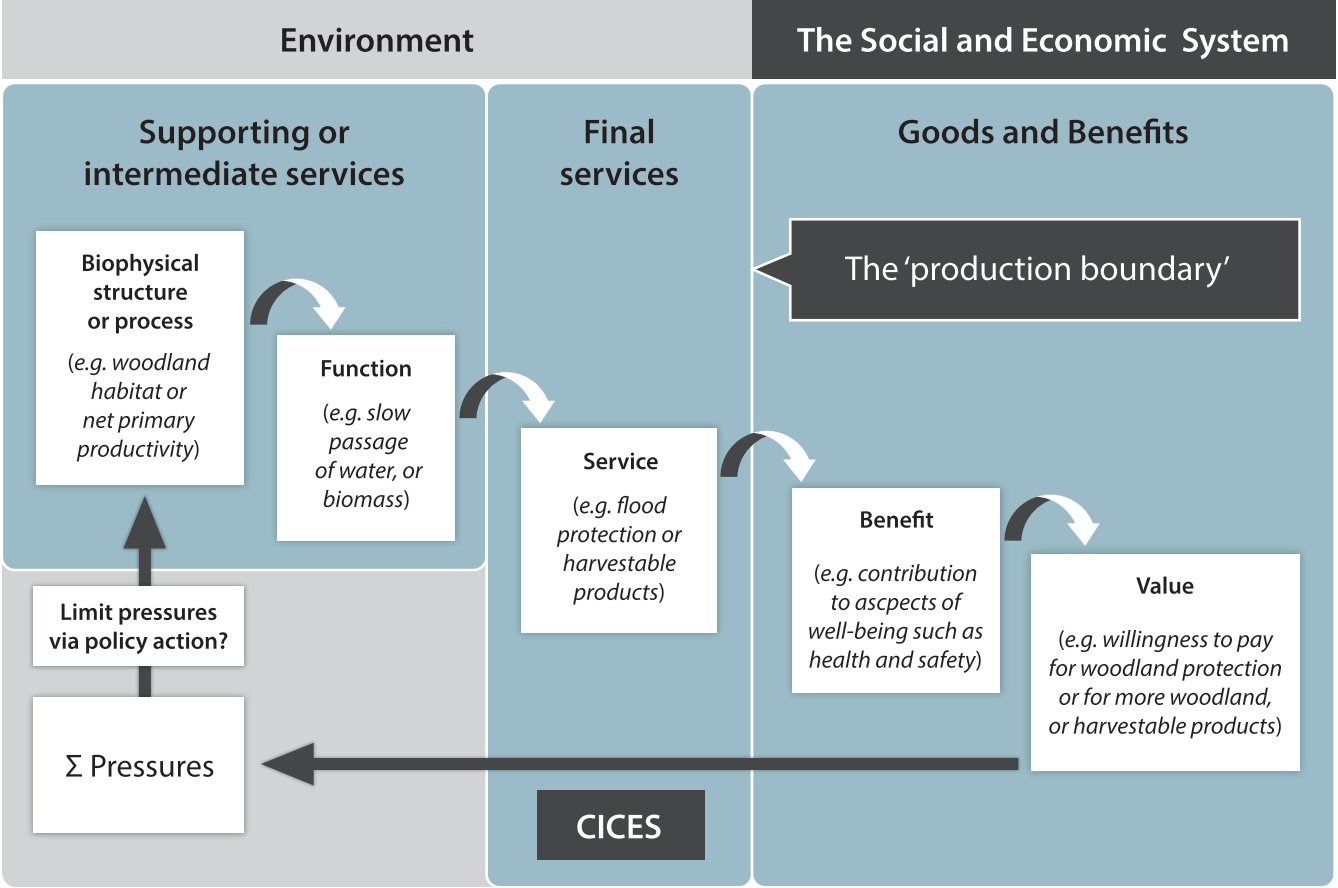
\includegraphics[width=1\linewidth]{/Users/fabio/Documents/4-Projects/everest-bio/PubliER/Figures/Potschin-Burkhard2017} 

}

\caption{ES conceptual framework}(\#fig:Fig:ES)
\end{figure}

In the context of this article, the CICES approach is chosen by the fact that it establish hierarchically consistent and science-based classification to be used for natural capital accounting purposes.
\protect\hyperlink{ref-Potschin-Young2018}{Potschin-Young et al.} (\protect\hyperlink{ref-Potschin-Young2018}{2018}) argued the conceptual framework of `ecosystem service cascade' feature make it possible to re-frame the analysis of ES helping in the clarification of the complex relationships that can be placed.
CICES scheme refers to ES specifically as the products from ecosystem, which can be directly used by human-beings.
This implies that \emph{supporting services}, defined in MEA framework, are excluded from CICES scheme, by the fact that human beings do not `receive'consumed' directly the benefits of these services.
Additionally, it tries to avoid the double-counting problem.
In that sense, CICES has \emph{regulation and maintenance services} as one section only.
The other two are \emph{provisioning services} and \emph{cultural services}.
From there, there are \emph{Divisions} describing the main types of output or process, and these are further split into \emph{groups} according to biological, physical or cultural type or process.
The lowest level is the \emph{class}, which specify the biological / material outputs and bio-physical and cultural processes.
Finally, the \emph{class type} measures the \emph{class level} which are the individual entities of the ESs.
Nevertheless, this cascade aspect is not far from critics.
(\protect\hyperlink{ref-Constanza2017}{\textbf{Constanza2017?}}) raised the point that the complex connections among the different ES and the benefits might be poorly represented by a linear `cascade' model, which assumes simple linkages and effects.
But on the other hand, the hierarchical structure can add different levels of detail needed by decision makers.

Figure \ref{fig:ES-CICES} presents the whole structure of ES from the CICES V5.1 {[}@{]}

\begin{figure}[!ht]

{\centering 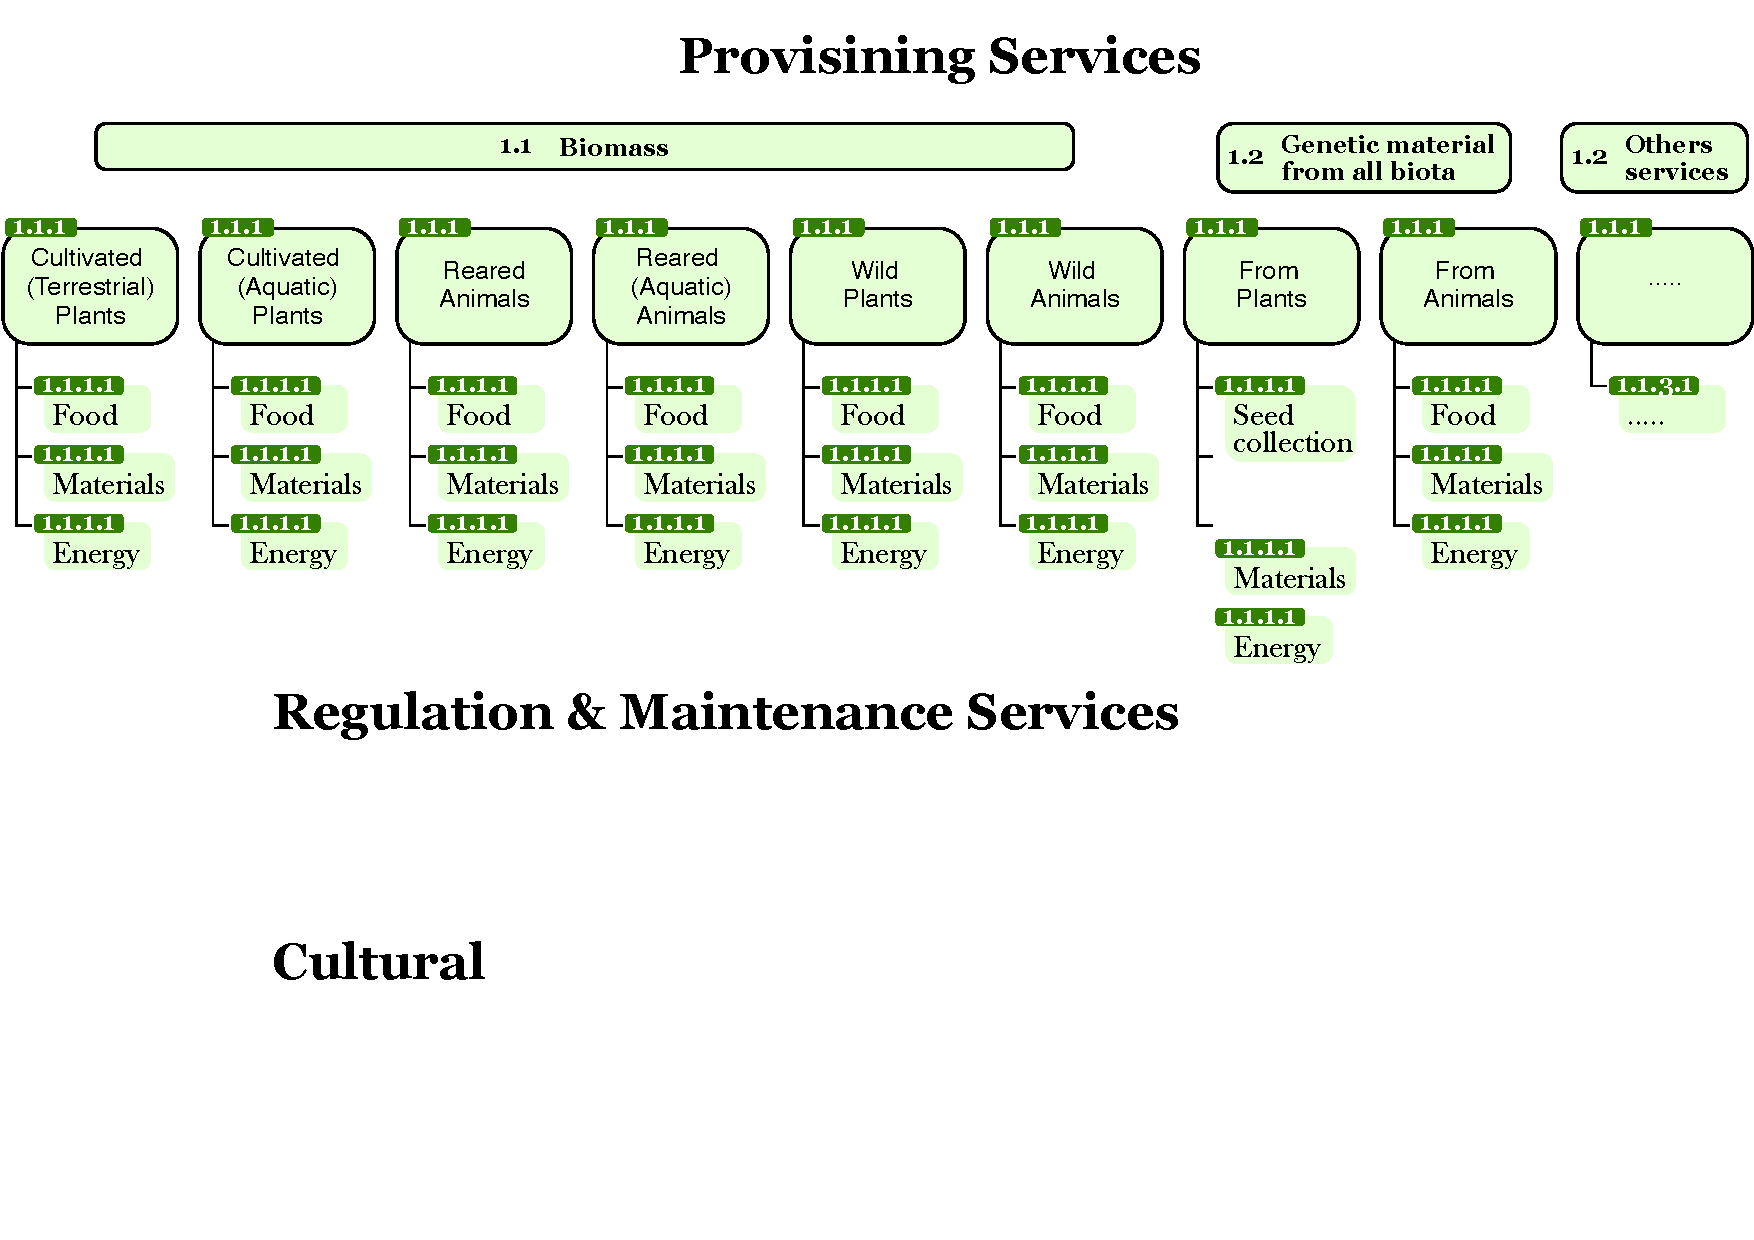
\includegraphics[width=1\linewidth]{/Users/fabio/Documents/4-Projects/everest-bio/PubliER/Figures/CICES-diagram} 

}

\caption{ES conceptual framework}\label{fig:ES-CICES}
\end{figure}

\hypertarget{ecosystems-services-and-industrial-systems-towards-a-synergy-between-both}{%
\subsection{Ecosystems services and industrial systems: Towards a synergy between both}\label{ecosystems-services-and-industrial-systems-towards-a-synergy-between-both}}

In environmental management, major efforts have been dedicated to the evaluation of the environmental impact of industrial systems using Life cycle assessment (LCA).
LCA aims to assess impacts on ecosystems, natural resources, and human health, as three primary areas of protection.
LCA proffers an internationally standardized approach to modeling, assessing, and valuing the impacts of a product or process throughout its life cycle.
However, a design approaches based on life cycle characterization and footprint methods focus on continuous improvement by reducing life cycle impacts per unit of product, encouraging improvements by doing ``less bad,'' which need not necessary translate into keeping human activities within ecological constraints.
Moreover, LCA does not fully acknowledge impacts on the supply of ES.
Assessing the impacts of production systems on ES supply is a new -- and contested -- paradigm of the latest years (\protect\hyperlink{ref-Vanderwilde2021}{Vanderwilde and Newell, 2021})
Ideally, it is needed to (re)designed industrial activities to reduce the demand of ecosystems services creating for a local `\emph{island of sustainability}' (\protect\hyperlink{ref-Wallner1996}{Wallner et al., 1996}) which is that the demand should not exceed the supply at the local scale (\protect\hyperlink{ref-Gopalakrishnan2016}{Gopalakrishnan et al., 2016}).

Ecosystems services and industrial systems need to be confronted to holistic evaluation to determine the externalities positive and negative.
In particular, full cost accounting in the business and governmental sectors, including new comprehensive accounts that include both the negative impacts on ES from business activities and the positive contributions of ES to businesses and households are key to develop (\protect\hyperlink{ref-Costanza2017}{Costanza et al., 2017})
Decision makers at the early stages should take into account the potential synergies and threats that the development of industrial systems could have to the local ecosystems.
For instance, \protect\hyperlink{ref-Bakshi2015}{Bakshi et al.} (\protect\hyperlink{ref-Bakshi2015}{2015}) reported a framework of Techno-Ecological Synergy (TES) in order to expand the scope of the usual techno-centric perspectives.
The main point argued is that TES develops ways of enhancing synergies between a local scale manufacturing process and the land around it.
The final aims is to encourage a more robust analysis of technological and ecological systems at multiple spatial scales ranging from local (e.g.~for small systems such as a house and its yard, a manufacturing process and its site) to a larger scale systems that extend to consider the entire life cycle.

In that sense, \protect\hyperlink{ref-Vanderwilde2021}{Vanderwilde and Newell} (\protect\hyperlink{ref-Vanderwilde2021}{2021}) reported a systematic literature review revealing that a persistent division between the LCA and ES research communities.
They putted forward that there are LCA research has focus on one or a few ES, especially carbon balance, sequestration, and emissions.
Also, the work has prioritized regulation and maintenance and provisioning services, with work especially scarce on cultural services.
Likewise, \protect\hyperlink{ref-Rugani2019}{Rugani et al.} (\protect\hyperlink{ref-Rugani2019}{2019}) proposed an approach towards consensus building in the assessment of human activities' impacts on the provision of ES and their beneficial uses for human well-being. More specifically, to harmonize the cascade concept (\protect\hyperlink{ref-RoyHaines-Young2018}{Roy Haines-Young and Potschin, 2018}) from the ES literature and the cause- effect chain modelling used in LCIA.

\hypertarget{ecosystems-services-at-the-urban-territorial-planification}{%
\subsection{Ecosystems services at the urban territorial planification}\label{ecosystems-services-at-the-urban-territorial-planification}}

More than two thirds of the world's population are expected to live in cities by 2050 (\protect\hyperlink{ref-ref}{\textbf{ref?}}).
Thus, the integration of ecosystem services in the urban and peri-urban planning is a key issue for prioritizing the quality of life in cities (\protect\hyperlink{ref-Gomez-Baggethun2013}{Gómez-Baggethun and Barton, 2013}), helping to urban planners to guarantee that future city districts the local people have access to urban greenery and their services

Urban ecosystems are especially important in providing services with direct impact on health and security such as air purification, noise reduction, urban cooling, and runoff mitigation (\protect\hyperlink{ref-Bolund1999}{Bolund and Hunhammar, 1999}).
\protect\hyperlink{ref-Croci2021}{Croci et al.} (\protect\hyperlink{ref-Croci2021}{2021}) presented a critical review
\protect\hyperlink{ref-Gomez-Baggethun2013}{Gómez-Baggethun and Barton} (\protect\hyperlink{ref-Gomez-Baggethun2013}{2013}) draws on the developments of the ecosystem services for urban planning.
They formulated a classification of ecosystem services and disservices in urban areas, including valuation methods and tools.

Using this background on ES from the different perspectives, in the following section a methodology is proposed converge main ES that are relevant for the industrial, territorial and global value chain.

\hypertarget{methodology}{%
\section{Methodology}\label{methodology}}

\label{methodology}

The purpose of this article is to identify main relevant ES services from a industrial and territorial perspective at the early design of industrial systems.
This identification is a first step with the purpose to evaluate the supply and demand of ecosystem services for these industrial systems.

\begin{figure}[!ht]

{\centering 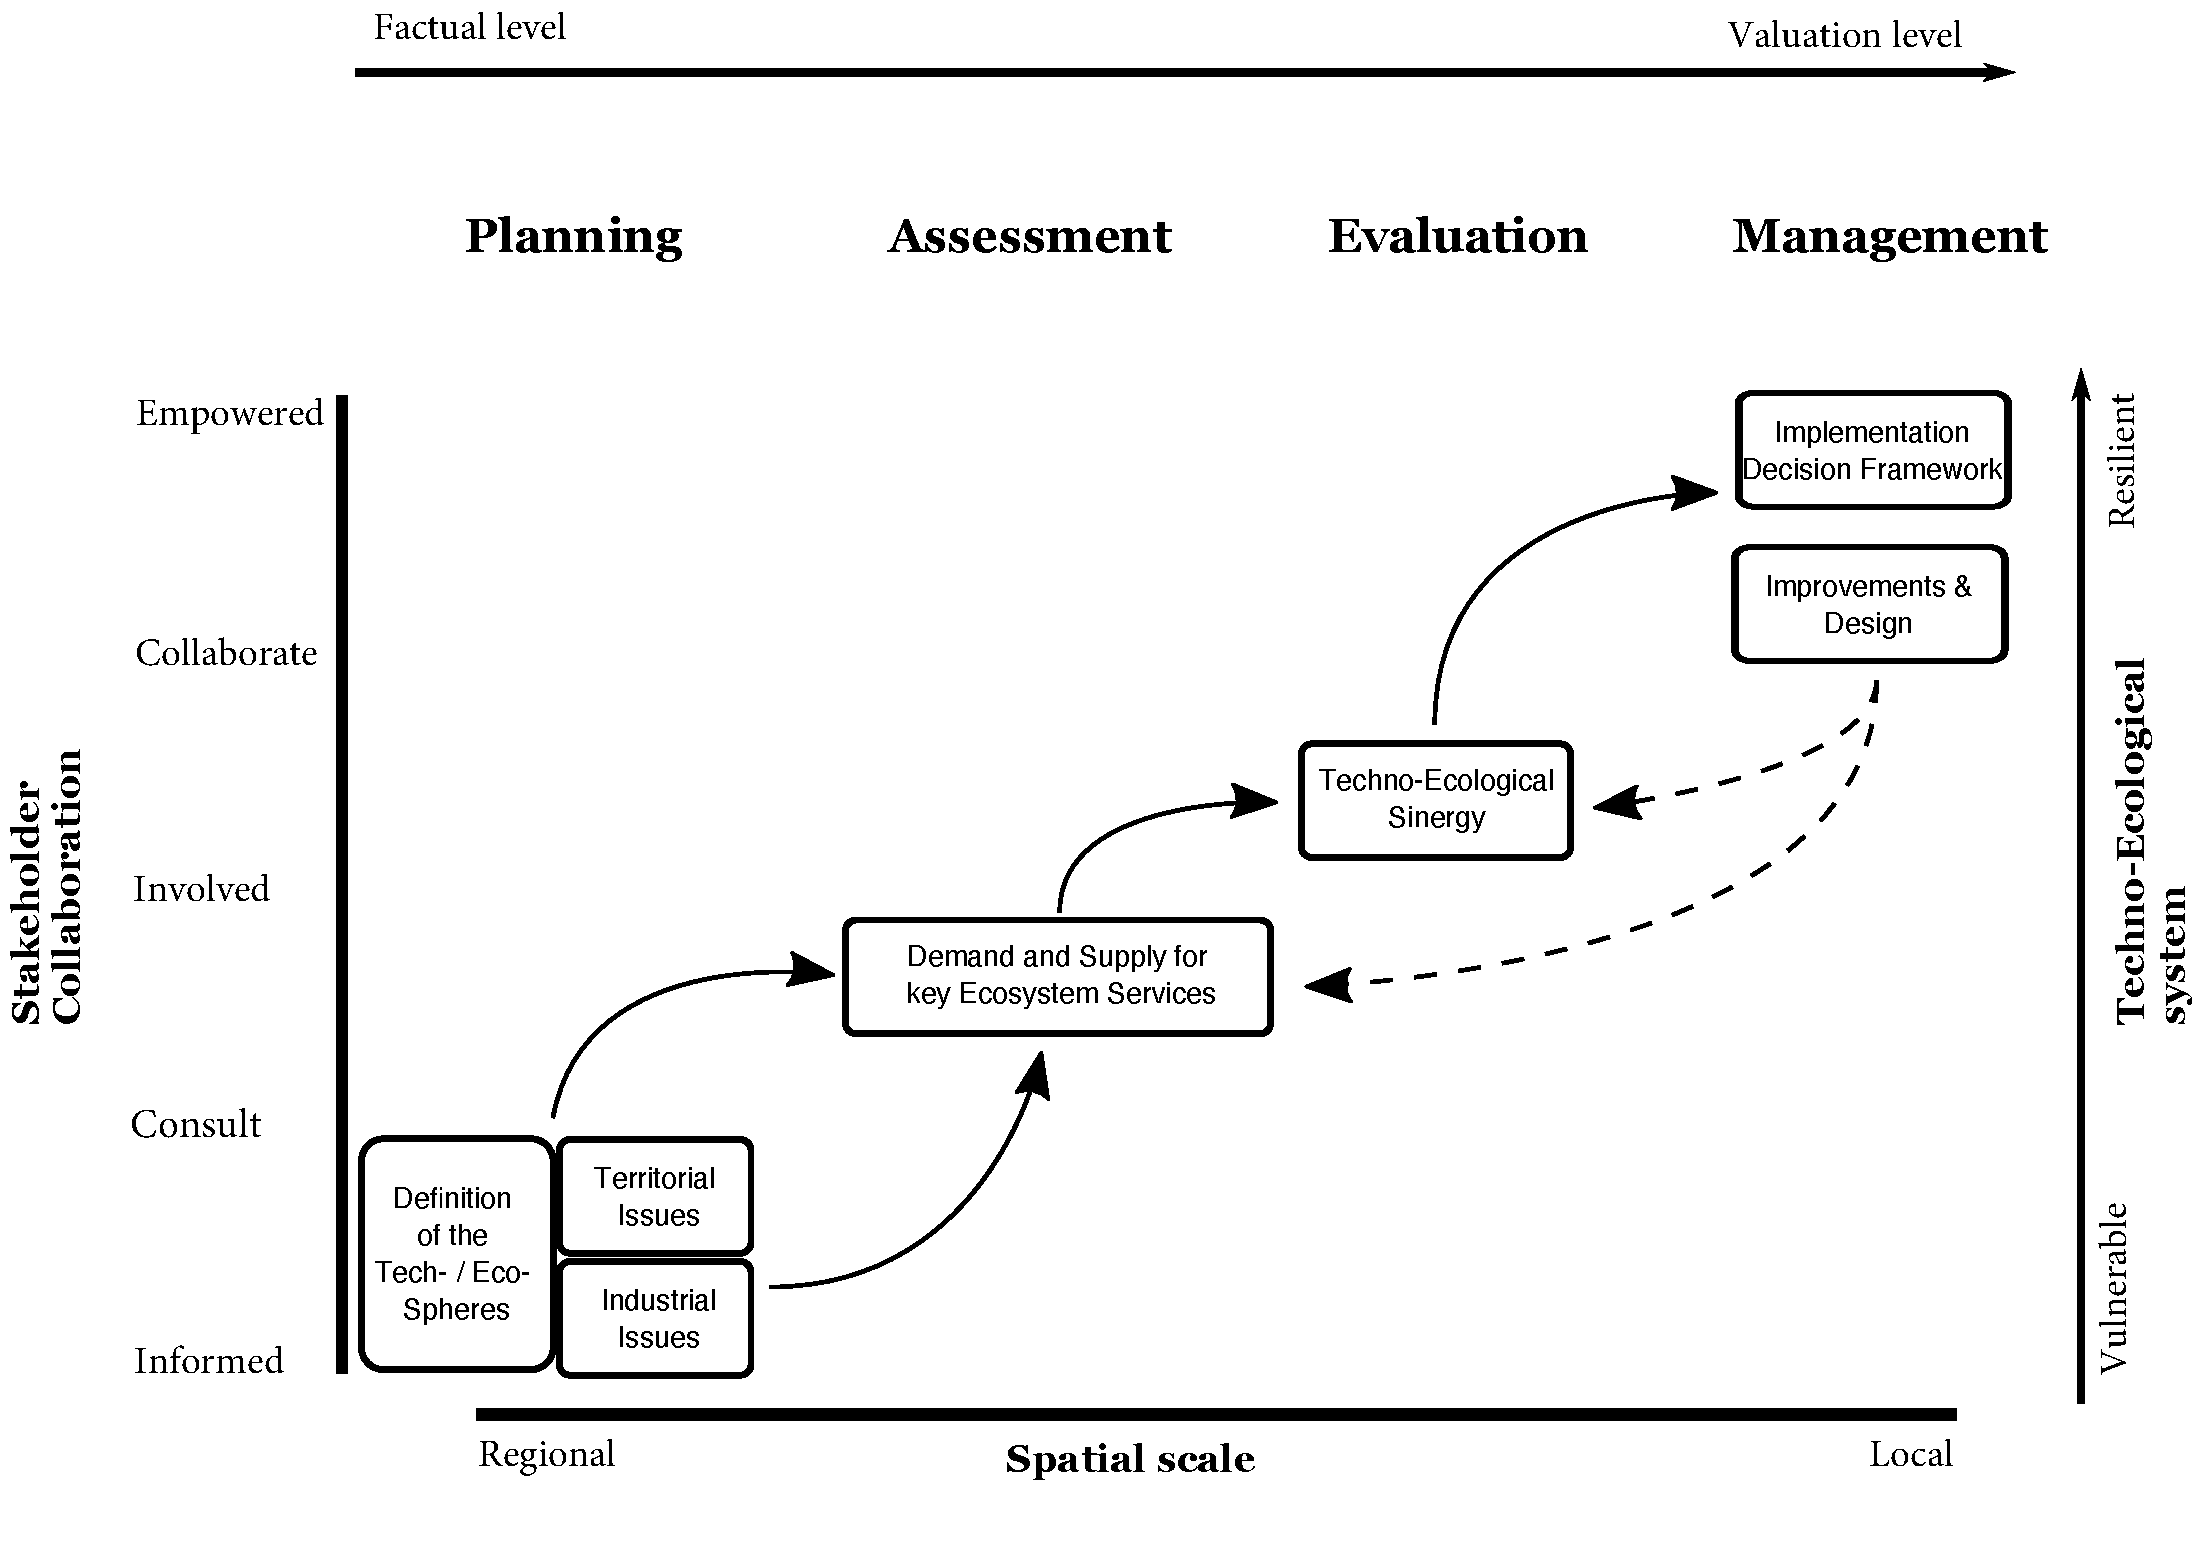
\includegraphics[width=1\linewidth]{/Users/fabio/Documents/4-Projects/everest-bio/PubliER/Figures/Methodology} 

}

\caption{Operational framework for evaluatig the ecosystem services of industrial systems}\label{fig:Fig-Methodology}
\end{figure}

Four major steps are proposed as illustrated in figure \ref{Fig-Methodology} .

\begin{itemize}
\item
  \textbf{I) Global value Planning}: the main goal is to identify the the links between the global value chain to be evaluated and the capital nature through the literature on ecological systems.
  The main purpose in this step is to map the the interactions positive and negative.
\item
  \textbf{II) Industrial system}: the main aim is to define the technosphere and identify the key ecosystems services that are impacted.
  The identification is made using the lens of connection between the LCA and ES elements.
\item
  \textbf{II) Industrial system}: in this step, the main purpose is the identification of the key urban priorities in the territorial context from a perspective of ecosystem services.
  To establish these priorities, the territorial planification perspective is analysed given the fact that a particular city varies greatly in function of the environmental and socio-economic characteristics of the territory.
\item
  Finally, in \textbf{IV) Synthesis}, the main goal is to converge on main ES that are identified for the three last perspectives,
\end{itemize}

In the following sub-sections, each stage of the methodology is explained.
An application of the framework will be presented in Section \label{results} using as case study of the distributed recycling chain via additive manufacturing.

\hypertarget{results}{%
\section{Results}\label{results}}

\label{results}

Context of the industrial system

A prospective distributed recycling chain for additive manufacturing .

\hypertarget{step-i---ecosystem-services-issues-at-the-value-chain-plastic-issues-at-the-ecosystems}{%
\subsection{Step I - Ecosystem Services issues at the Value chain: Plastic issues at the ecosystems}\label{step-i---ecosystem-services-issues-at-the-value-chain-plastic-issues-at-the-ecosystems}}

The goal of this first step is to highlight the main interactions that the value chain have with the natural ecosystems.
This enables us to have a holistic picture of the impacts of plastic pollution in the natural ecosystems taking into account the highlighting the uncertainties and knowledge gaps that could exist in the field.

\begin{figure}

{\centering 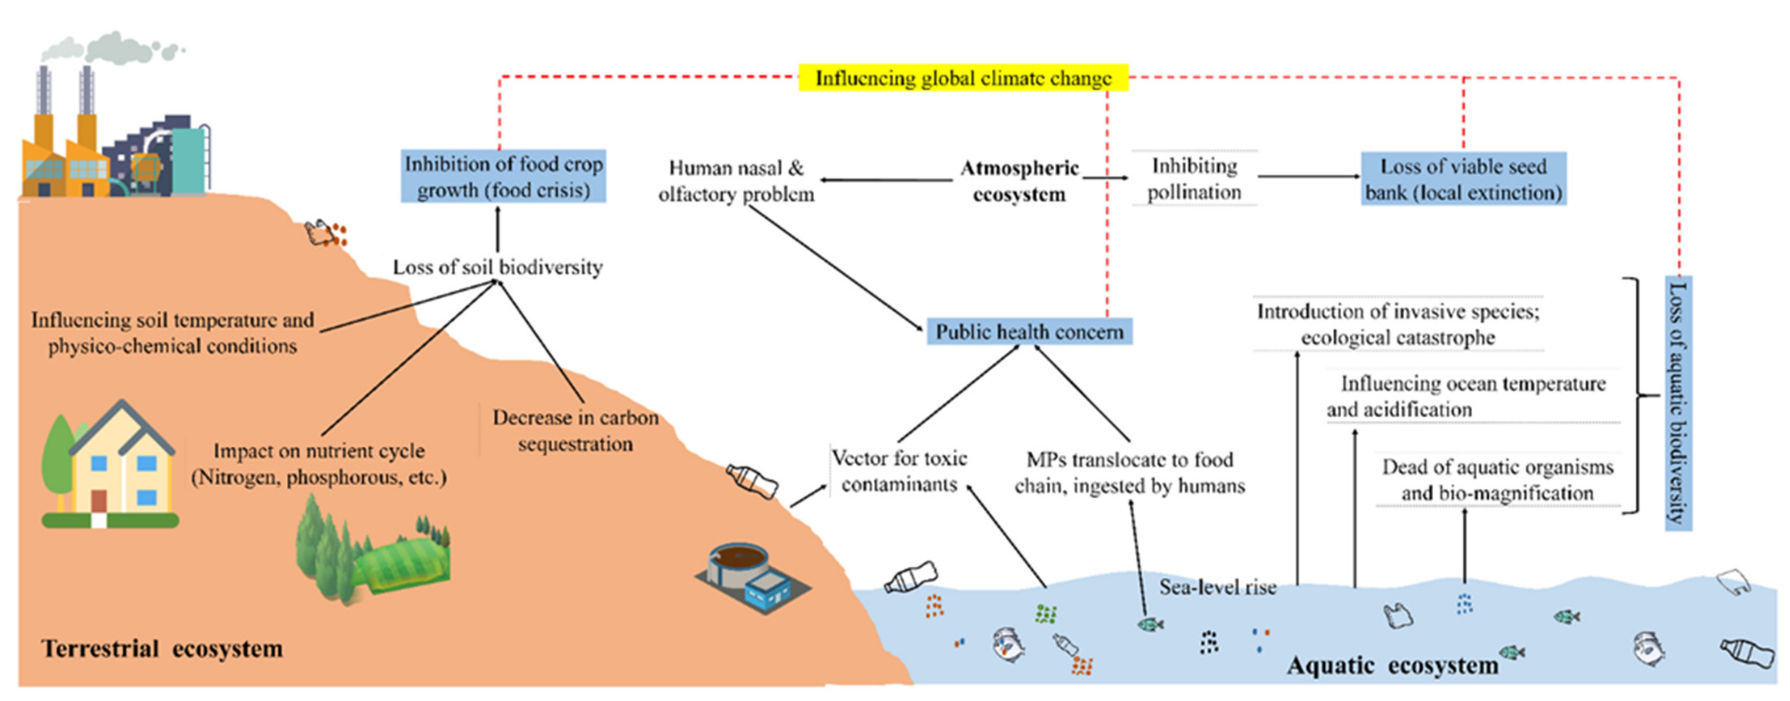
\includegraphics[width=1\linewidth]{/Users/fabio/Documents/4-Projects/everest-bio/PubliER/Figures/Kumar2021} 

}

\caption{Illustration of MPs and NPs affecting various ecosystem services and climate change on terrestrial, aquatic, and atmospheric ecosystems. Source. Kumar2021.jpg}\label{fig:fig-Kumar2021}
\end{figure}

\protect\hyperlink{ref-Kumar2021}{Kumar et al.} (\protect\hyperlink{ref-Kumar2021}{2021}) reported a complete description of the major impacts on the plastic pollution an the ecosystems services,identifying in what extend there are present the interlinkages between plastic pollution, waste management, and Sustainable Development Goals (SDG).
Figure \ref{fig:fig-Kumar2021} presents an overview of the major interactions that plastic impact the ecosystem services in the terrestrial and aquatic ecosystems, representing a major societal issue.
Macrosplastics -MP- (particules \(\geq 5mm\) ), mesoplastics -MsP- (\(1-5 mm\)) and microplastics (\(<1~mm\)) are the major problems in the ecosystems.

For aquatic ecosystems, main risks are linked to standing water that acts as a breeding niche (to mosquitoes, pests, vector-borne diseases transmission), becomes a vector for toxic chemicals and, ultimately, disturbs the natural cycles (biogeochemical cycle in terrestrial ecosystems). Additionally, the transfer of plastic into the food chain is a clear danger to animal and, certainly, to humans as well. Thus, reducing the consumption of plastics is of great importance in the long term.

The plastic value chain is one of the mo

\begin{itemize}
\item
  Plastic materials have impats on the terrestrial, qauqtic, and atmospheric ecosystems.
\item
\end{itemize}

Concerning the terrestrial impacts, the plastic degradation make and important impact on the pollitation of the

The global value chain of the plastic material

\renewcommand{\arraystretch}{1.5}

\begin{longtable}[]{@{}
  >{\raggedright\arraybackslash}p{(\columnwidth - 4\tabcolsep) * \real{0.68}}
  >{\raggedright\arraybackslash}p{(\columnwidth - 4\tabcolsep) * \real{0.10}}
  >{\raggedright\arraybackslash}p{(\columnwidth - 4\tabcolsep) * \real{0.22}}@{}}
\toprule
\begin{minipage}[b]{\linewidth}\raggedright
Description
\end{minipage} & \begin{minipage}[b]{\linewidth}\raggedright
ES impact
\end{minipage} & \begin{minipage}[b]{\linewidth}\raggedright
Ref
\end{minipage} \\
\midrule
\endhead
Soil productivity is impacted due to the nutrient imbalance followed by oxidative stress and leading to the poor growth of food crops & 1.1.1.1 ; 1.2.1.1 ~~~~~ & (\protect\hyperlink{ref-Garcia-Vazquez2021}{Garcia-Vazquez and Garcia-Ael, 2021}; \protect\hyperlink{ref-Kumar2021}{Kumar et al., 2021}) \\
~~~~~~ ~~~~~~ & & \\
MPs and their suspended solids hasten eutrophication adding more contaminants to the food chain supply and primarily creating organic contamination. & 1.1.5.1 ; 1.1.6.1 & {[}136{]} \\
MPs and NPs in the atmosphere also lead to the obstruction and lowering of pollination. & 2.2.2.1 & (\protect\hyperlink{ref-Kumar2021}{Kumar et al., 2021}) \\
MPs and NPs are established to act as a vector and breach through any system (organisms) and even via trophic transfer (one trophic level to another via food chain), therefore, it can be hypothesized that MPs in the future can play a pivotal role in the spill over of infectious diseases, leading to an epidemic or pandemic of unknown scale & 2.2.3.1; 2.2.3.1 & Ref \\
MP and NP in terrestrial ecosystems reduce tha ability to sequester carbon. & 2.1.1.2 ; 2.2.4.1 & (\protect\hyperlink{ref-Kumar2021}{Kumar et al., 2021}) \\
Elements as nitrogen and phosphorous, are also vividly influenced due to MPs and NPs in the soil ecosystem & 2.2.4.1 ; 2.2.4.2 & (\protect\hyperlink{ref-Kumar2021}{Kumar et al., 2021}) \\
MPs accumulation can promote mineralization, nitrification, and denitrification in aquatic ecosystems, therefore releasing CO2, CH4, and N2O. & 2.2.6.1 & (\protect\hyperlink{ref-Kumar2021}{Kumar et al., 2021}) \\
marine carbon sinks are critical in analyzing the global climate change and are potentially affected by MPs and NPs pollution on phytoplankton-sequestered CO2 and their transmission to the deep ocean via zooplankton {[}77{]}. & 2.2.5.2 & (\protect\hyperlink{ref-Kumar2021}{Kumar et al., 2021}) \\
Plastics-induced variations in solar radiation in the water column can alter physical processes at the ocean's surface and near-surface layers as well as trigger climate feedback mechanisms & 2.2.6.1 & (\protect\hyperlink{ref-Kumar2021}{Kumar et al., 2021}) \\
MPs and NPs are known to cause a dynamic shift in the soil temperature as is commonly practiced in agriculture sectors with extreme climatic conditions. & 2.2.4.1 & \\
MPs and NPs in the soil ecosystem are known to have a strong impact on the population structure and survival of these faunas {[}135,137,154,158{]}. & 2.2.4.1 & \\
Small-sized plastics act as stressors, altering the ocean level and temperature and influencing the acidification. & 2.2.6.1 & \\
High amounts of MPs and NPs are more substantially found in pelagic species than in deep-water species. & 1.1.5.1 & \\
MPs and NPs act as vectors for toxic chemicals and microbes and can breach any ecosystem. & 2.1.1.1 & REf \\
\bottomrule
\end{longtable}

\hypertarget{step-ii---definition-the-industrial-system-distributed-recycling-via-additive-manufacturing}{%
\subsection{Step II - Definition the Industrial system : Distributed recycling via additive manufacturing}\label{step-ii---definition-the-industrial-system-distributed-recycling-via-additive-manufacturing}}

Major technological advances in the additive manufacturing (AM) field have enable the validation of distributed fabrication (\protect\hyperlink{ref-Matt2015}{Matt et al., 2015}; \protect\hyperlink{ref-Petersen2017a}{Petersen and Pearce, 2017}; \protect\hyperlink{ref-Woern2017}{Woern and Pearce, 2017}).
In the same logic, recently, the concept of distributed recycling via additive manufacturing (DRAM) emerged in the literature to face the technico-environmental challenges related to recycling option, mostly for material-extrusion based technologies using thermoplastic assets as feedstock (\protect\hyperlink{ref-CruzSanchez2020}{Cruz Sanchez et al., 2020}; \protect\hyperlink{ref-Santander2020}{Santander et al., 2020}).
The use of recycled material, either in the form of raw material or blended with virgin material, is a method of special interest to contribute to sustainable manufacturing (\protect\hyperlink{ref-Zhao2018}{Zhao et al., 2018}).

The main hypothesis relies on the fact that a distributed and local spaces can provide recycled feedstock to transform it into finish (or prototypes) for a local community.
To do so, the use of additive manufacturing enables the technical paths to achieve this objective.
In the DRAM methodology, consumers have an economic incentive to recycle.
This is because they can use their waste as feedstock for a wide range of consumer products that can be produced for a fraction of the conventional cost of the equivalent products.
Moreover, 3D printing is especially well suited because it enables the production of parts with (almost) no waste, and could reduce the waste related to the material by more than 40 \%, reusing 95 \% of the unused material (\protect\hyperlink{ref-Petrovic2011}{Petrovic et al., 2011}).
Currently, most of the cost of 3D printing is associated with filament in FFF techniques (\protect\hyperlink{ref-Wittbrodt2013}{Wittbrodt et al., 2013}).

By recycling raw materials such as Polylactic acid (PLA), one of the most frequently used materials in 3D printing, it is possible to reduce the carbon dioxide emissions that are incurred by transport to landfills or shipping to customers, offering environmental benefits (\protect\hyperlink{ref-Santander2020}{Santander et al., 2020}).

However, while not all types of materials can be recycled given the technical difficulties, the integral evaluation of the environmental advantage is needed to assess at early stages the pertinence of this distributed approaches.
Although research has been conducted regarding on the technical and logistical feasibility of distributed plastic recycling, little is known about its pertinence from the ecosystem services perspective in a territory.

The technical system is depicted in the figure XX.

From a perspective of AM process, several researches have used the life cycle impact assessment (LCIA) for the case of distributed recycling (\protect\hyperlink{ref-Garcia2021}{Garcia et al., 2021}; \protect\hyperlink{ref-Kerdlap2021}{Kerdlap et al., 2021}; \protect\hyperlink{ref-Kreiger2014}{Kreiger et al., 2014}; \protect\hyperlink{ref-Kreiger2013}{Kreiger and Pearce, 2013}; \protect\hyperlink{ref-Zhao2018}{Zhao et al., 2018}).
The main element to highlight is that climate change (global warming potential -GWP-) and cumulative energy demand (CED) are the most studied impact factors in the literature of additive manufacturing.
For instance, using a technical system \emph{recyclebot} to create 3D printing recycled filament with High Density Polyethylen (HPDE),
\protect\hyperlink{ref-Kreiger2014}{Kreiger et al.} (\protect\hyperlink{ref-Kreiger2014}{2014}) argued that the distributed recycling can decrease the embodied energy by 69\%-82\% with respect to conventional recycling using CED estimations.
\protect\hyperlink{ref-Zhao2018}{Zhao et al.} (\protect\hyperlink{ref-Zhao2018}{2018}) estimated the environmental impacts associated with disposal of 1 kg PLA in three end-of-life options (landfill, recycling, incineration), making a point that recycling option is made using 3D printing technology.
They used GWP (in kg CO2 eq), ozone depletion potential (ODP, in CFC-11 eq), fossil depletion potential (FDP, in kg oil eq), human toxicity potential (HTP, in kg 1,4-DB eq), particulate matter formation potential (PMFP, in kg PM10 eq), photochemical oxidant formation potential (POFP, in kg NMVOC), freshwater eutrophication potential (FEP, in kg P eq), freshwater ecotoxicity potential (FETP, in kg 1,4-DB eq), marine eutrophication potential (MEP, in kg N eq), marine ecotoxicity potential (METP, in kg 1,4-DB eq), terrestrial acidification potential (TAP, in kg SO2 eq), and terrestrial ecotoxicity potential (TETP, in kg 1,4-DB eq).
In a more network level, \protect\hyperlink{ref-Kerdlap2021}{Kerdlap et al.} (\protect\hyperlink{ref-Kerdlap2021}{2021}) quantify the LCIA of distributed versus centralized plastic recycling systems of small-scale distributed plastic sorting and recycling systems in comparison to traditional large-scale centralized systems in Singapore. They used climate change and cumulative energy, water depletion and terrestrial eco-toxicity as impact categories.

Given these literature, it is possible to conclude that GWP and

\protect\hyperlink{ref-Vanderwilde2021}{Vanderwilde and Newell} (\protect\hyperlink{ref-Vanderwilde2021}{2021}) studied the connection of LCIA with the field of ecosystem services.
One major point from this studied is the proposition of the links that can connect the LCIA mid-point categories with the set of ES .
Nevertheless, they used the version.

Therefore, based on, table @ref

\begin{table}[!h]

\caption{\label{tab:unnamed-chunk-2}LCA impact categories of DRAM connecting with ES}
\centering
\begin{tabular}[t]{>{\raggedright\arraybackslash}p{10em}>{\raggedright\arraybackslash}p{30em}l}
\toprule
Description & ES & Ref\\
\midrule
\cellcolor{gray!6}{Climate change} & \cellcolor{gray!6}{2.2.4.1; 2.1.1.2; 2.2.4.1; 2.2.4.2} & \cellcolor{gray!6}{}\\
Eutrophication & 2.2.5.1; 2.2.5.2; 2.1.1.1; 2.1.1.2 & \\
\cellcolor{gray!6}{Ressources Depletion} & \cellcolor{gray!6}{All CICES-defined Provisioning (1.1.1.1 - 1.2.2.3; ) ES as potentially relevant; adding water availability (2.2.1.3; 2.2.5.1; 2.2.5.2} & \cellcolor{gray!6}{}\\
\bottomrule
\end{tabular}
\end{table}

\hypertarget{step-iii---ecosystem-services-priorities-at-the-territorial-level-nancy-france}{%
\subsection{Step III - Ecosystem services Priorities at the territorial level: Nancy, France}\label{step-iii---ecosystem-services-priorities-at-the-territorial-level-nancy-france}}

In this step, the main goal is to identify the stratic axis that the territory put in the view of preserving/improving/restauring ecosystem services.
For that, we delimitate the city of Nancy, in the east region of , .

Based on the three main perspectives of ES,

\begin{itemize}
\item
  https://fr.calameo.com/read/005820422f7f4ab30f35b?page=1
\item
  https://www.ecologie.gouv.fr/levaluation-francaise-des-ecosystemes-et-des-services-ecosystemiques\#scroll-nav\_\_2
\item
  https://www.ecologie.gouv.fr/levaluation-francaise-des-ecosystemes-et-des-services-ecosystemiques\#scroll-nav\_\_3
\end{itemize}

\begin{table}[!h]

\caption{(\#tab:Tab:Nancy-ES)LCA impact categories of DRAM connecting with ES}
\centering
\begin{tabular}[t]{>{\raggedright\arraybackslash}p{10em}>{\raggedright\arraybackslash}p{30em}l}
\toprule
Description & ES & Ref\\
\midrule
\cellcolor{gray!6}{Clima - Air} & \cellcolor{gray!6}{2.2.6.1; 2.1.2.2} & \cellcolor{gray!6}{Calameo}\\
Sol & 2.2.4.1; 2.2.4.2 & Calameo\\
\bottomrule
\end{tabular}
\end{table}

\hypertarget{step-iv---identifying-the-hot-spot-of-the-es-for-the-case-of-dram-at-nancy-france}{%
\subsection{Step IV - Identifying the Hot spot of the ES for the case of DRAM at Nancy, France}\label{step-iv---identifying-the-hot-spot-of-the-es-for-the-case-of-dram-at-nancy-france}}

\begin{landscape}
\begin{figure}

{\centering 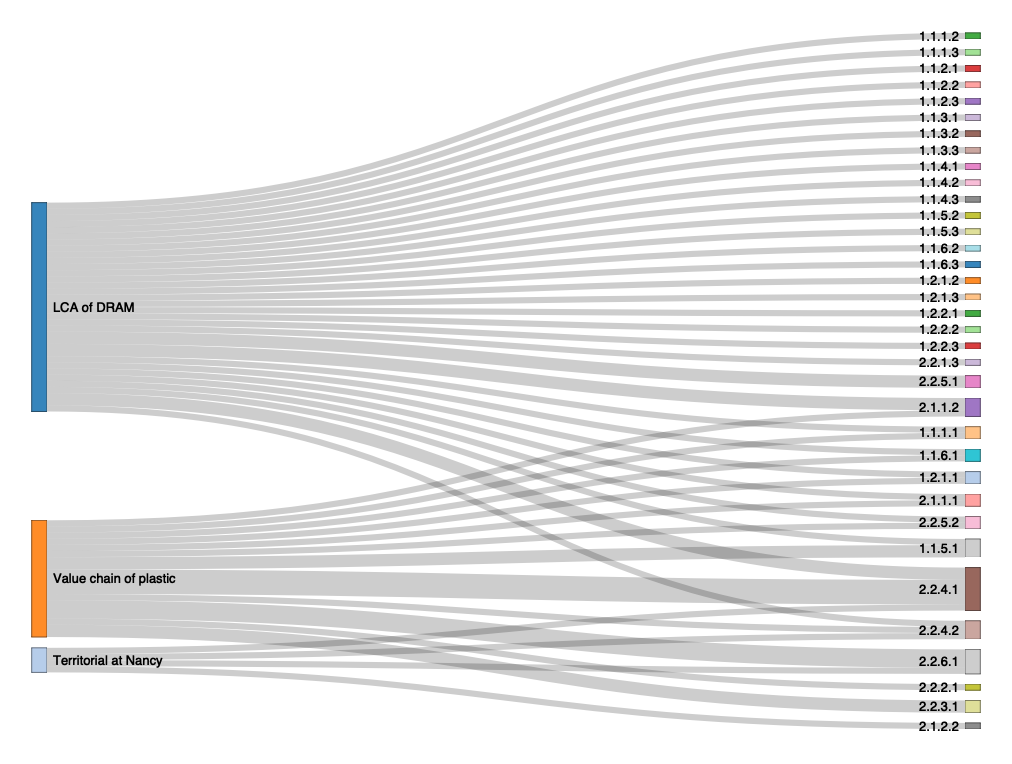
\includegraphics[width=1\linewidth]{/Users/fabio/Documents/4-Projects/everest-bio/PubliER/Figures/Sankey} 

}

\caption{Priorization of ES for the distributed recycling indsutrail system.}\label{fig:fig-sankey}
\end{figure}
\end{landscape}

\hypertarget{discussion-and-perspective-of-the-analysis}{%
\section{Discussion and perspective of the analysis}\label{discussion-and-perspective-of-the-analysis}}

\hypertarget{conclusions}{%
\section{Conclusions}\label{conclusions}}

\bibliography{library.bib}

\newpage

\hypertarget{references}{%
\section*{References}\label{references}}
\addcontentsline{toc}{section}{References}

\hypertarget{refs}{}
\begin{CSLReferences}{1}{0}
\leavevmode\vadjust pre{\hypertarget{ref-Abson2014}{}}%
Abson, D.J., Wehrden, H. von, Baumgärtner, S., Fischer, J., Hanspach, J., Härdtle, W., Heinrichs, H., Klein, A.M., Lang, D.J., Martens, P., Walmsley, D., 2014. {Ecosystem services as a boundary object for sustainability}. \url{https://doi.org/10.1016/j.ecolecon.2014.04.012}

\leavevmode\vadjust pre{\hypertarget{ref-Bakshi2019a}{}}%
Bakshi, B.R., 2019. {Toward sustainable chemical engineering: The role of process systems engineering}. \url{https://doi.org/10.1146/annurev-chembioeng-060718-030332}

\leavevmode\vadjust pre{\hypertarget{ref-Bakshi2018}{}}%
Bakshi, B.R., Gutowski, T.G., Sekulic, D.P., 2018. {Claiming Sustainability: Requirements and Challenges}. ACS Sustain. Chem. Eng. 6, 3632--3639. \url{https://doi.org/10.1021/acssuschemeng.7b03953}

\leavevmode\vadjust pre{\hypertarget{ref-Bakshi2015}{}}%
Bakshi, B.R., Ziv, G., Lepech, M.D., 2015. {Techno-Ecological Synergy: A Framework for Sustainable Engineering}. Environ. Sci. Technol. 49, 1752--1760. \url{https://doi.org/10.1021/es5041442}

\leavevmode\vadjust pre{\hypertarget{ref-Bolund1999}{}}%
Bolund, P., Hunhammar, S., 1999. {Ecosystem services in urban areas}. Ecol. Econ. 29, 293--301. \url{https://doi.org/10.1016/S0921-8009(99)00013-0}

\leavevmode\vadjust pre{\hypertarget{ref-Bruel2018}{}}%
Bruel, A., Kronenberg, J., Troussier, N., Guillaume, B., 2019. {Linking Industrial Ecology and Ecological Economics: A Theoretical and Empirical Foundation for the Circular Economy}. J. Ind. Ecol. 23, 12--21. \url{https://doi.org/10.1111/jiec.12745}

\leavevmode\vadjust pre{\hypertarget{ref-Bruel2016}{}}%
Bruel, A., Troussier, N., Guillaume, B., Sirina, N., 2016. {Considering Ecosystem Services in Life Cycle Assessment to Evaluate Environmental Externalities}. Procedia CIRP 48, 382--387. \url{https://doi.org/10.1016/j.procir.2016.03.143}

\leavevmode\vadjust pre{\hypertarget{ref-Ceschin2016}{}}%
Ceschin, F., Gaziulusoy, I., 2016. {Evolution of design for sustainability: From product design to design for system innovations and transitions}. Des. Stud. 47, 118--163. \url{https://doi.org/10.1016/j.destud.2016.09.002}

\leavevmode\vadjust pre{\hypertarget{ref-Costanza1997}{}}%
Costanza, R., D'Arge, R., Groot, R. de, Farber, S., Grasso, M., Hannon, B., Limburg, K., Naeem, S., O'Neill, R.V., Paruelo, J., Raskin, R.G., Sutton, P., Belt, M. van den, 1997. {The value of the world's ecosystem services and natural capital}. Nature 387, 253--260. \url{https://doi.org/10.1038/387253a0}

\leavevmode\vadjust pre{\hypertarget{ref-Costanza2017}{}}%
Costanza, R., Groot, R. de, Braat, L., Kubiszewski, I., Fioramonti, L., Sutton, P., Farber, S., Grasso, M., 2017. {Twenty years of ecosystem services: How far have we come and how far do we still need to go?} \url{https://doi.org/10.1016/j.ecoser.2017.09.008}

\leavevmode\vadjust pre{\hypertarget{ref-Croci2021}{}}%
Croci, E., Lucchitta, B., Penati, T., 2021. {Valuing ecosystem services at the urban level: A critical review}. \url{https://doi.org/10.3390/su13031129}

\leavevmode\vadjust pre{\hypertarget{ref-CruzSanchez2020}{}}%
Cruz Sanchez, F.A., Boudaoud, H., Camargo, M., Pearce, J.M., 2020. {Plastic recycling in additive manufacturing: A systematic literature review and opportunities for the circular economy}. J. Clean. Prod. 264, 121602. \url{https://doi.org/10.1016/j.jclepro.2020.121602}

\leavevmode\vadjust pre{\hypertarget{ref-DeGroot2002}{}}%
De Groot, R.S., Wilson, M.A., Boumans, R.M.J., 2002. {A typology for the classification, description and valuation of ecosystem functions, goods and services}. Ecol. Econ. 41, 393--408. \url{https://doi.org/10.1016/S0921-8009(02)00089-7}

\leavevmode\vadjust pre{\hypertarget{ref-Diwekar2021}{}}%
Diwekar, U., Amekudzi-Kennedy, A., Bakshi, B., Baumgartner, R., Boumans, R., Burger, P., Cabezas, H., Egler, M., Farley, J., Fath, B., Gleason, T., Huang, Y., Karunanithi, A., Khanna, V., Mangan, A., Mayer, A.L., Mukherjee, R., Mullally, G., Rico-Ramirez, V., Shonnard, D., Svanström, M., Theis, T., 2021. {A perspective on the role of uncertainty in sustainability science and engineering}. Resour. Conserv. Recycl. 164, 105140. \url{https://doi.org/10.1016/j.resconrec.2020.105140}

\leavevmode\vadjust pre{\hypertarget{ref-Ekins2003}{}}%
Ekins, P., Simon, S., Deutsch, L., Folke, C., De Groot, R., 2003. {A framework for the practical application of the concepts of critical natural capital and strong sustainability}. Ecol. Econ. 44, 165--185. \url{https://doi.org/10.1016/S0921-8009(02)00272-0}

\leavevmode\vadjust pre{\hypertarget{ref-Garcia2021}{}}%
Garcia, F.L., Nunes, A.O., Martins, M.G., Belli, M.C., Saavedra, Y.M.B., Silva, D.A.L., Moris, V.A. da S., 2021. {Comparative LCA of conventional manufacturing vs. additive manufacturing: the case of injection moulding for recycled polymers}. Int. J. Sustain. Eng. 00, 1--19. \url{https://doi.org/10.1080/19397038.2021.1990435}

\leavevmode\vadjust pre{\hypertarget{ref-Garcia-Vazquez2021}{}}%
Garcia-Vazquez, E., Garcia-Ael, C., 2021. {The invisible enemy. Public knowledge of microplastics is needed to face the current microplastics crisis}. Sustain. Prod. Consum. 28, 1076--1089. \url{https://doi.org/10.1016/j.spc.2021.07.032}

\leavevmode\vadjust pre{\hypertarget{ref-Gomez-Baggethun2013}{}}%
Gómez-Baggethun, E., Barton, D.N., 2013. {Classifying and valuing ecosystem services for urban planning}. Ecol. Econ. 86, 235--245. \url{https://doi.org/10.1016/j.ecolecon.2012.08.019}

\leavevmode\vadjust pre{\hypertarget{ref-Gomez-Baggethun2010}{}}%
Gómez-Baggethun, E., Groot, R. de, Lomas, P.L., Montes, C., 2010. {The history of ecosystem services in economic theory and practice: From early notions to markets and payment schemes}. Ecol. Econ. 69, 1209--1218. \url{https://doi.org/10.1016/j.ecolecon.2009.11.007}

\leavevmode\vadjust pre{\hypertarget{ref-Gopalakrishnan2016}{}}%
Gopalakrishnan, V., Bakshi, B.R., Ziv, G., 2016. {Assessing the capacity of local ecosystems to meet industrial demand for ecosystem services}. AIChE J. 62, 3319--3333.

\leavevmode\vadjust pre{\hypertarget{ref-Harrison2018}{}}%
Harrison, P.A., Dunford, R., Barton, D.N., Kelemen, E., Martín-López, B., Norton, L., Termansen, M., Saarikoski, H., Hendriks, K., Gómez-Baggethun, E., Czúcz, B., García-Llorente, M., Howard, D., Jacobs, S., Karlsen, M., Kopperoinen, L., Madsen, A., Rusch, G., Van Eupen, M., Verweij, P., Smith, R., Tuomasjukka, D., Zulian, G., 2018. {Selecting methods for ecosystem service assessment: A decision tree approach}. Ecosyst. Serv. 29, 481--498. \url{https://doi.org/10.1016/j.ecoser.2017.09.016}

\leavevmode\vadjust pre{\hypertarget{ref-Honeck2021}{}}%
Honeck, E., Gallagher, L., Arx, B. von, Lehmann, A., Wyler, N., Villarrubia, O., Guinaudeau, B., Schlaepfer, M.A., 2021. {Integrating ecosystem services into policymaking -- A case study on the use of boundary organizations}. Ecosyst. Serv. 49, 101286. \url{https://doi.org/10.1016/j.ecoser.2021.101286}

\leavevmode\vadjust pre{\hypertarget{ref-IPBS2019}{}}%
IPBS, 2019. {Global assessment report on biodiversity and ecosystem services of the Intergovernmental Science-Policy Platform on Biodiversity and Ecosystem Services}.

\leavevmode\vadjust pre{\hypertarget{ref-Kerdlap2021}{}}%
Kerdlap, P., Purnama, A.R., Low, J.S.C., Tan, D.Z.L., Barlow, C.Y., Ramakrishna, S., 2021. {Comparing the environmental performance of distributed versus centralized plastic recycling systems: Applying hybrid simulation modeling to life cycle assessment}. J. Ind. Ecol. \url{https://doi.org/10.1111/jiec.13151}

\leavevmode\vadjust pre{\hypertarget{ref-Kreiger2014}{}}%
Kreiger, M.a., Mulder, M.L., Glover, A.G., Pearce, J.M., 2014. {Life cycle analysis of distributed recycling of post-consumer high density polyethylene for 3-D printing filament}. J. Clean. Prod. 70, 90--96. \url{https://doi.org/10.1016/j.jclepro.2014.02.009}

\leavevmode\vadjust pre{\hypertarget{ref-Kreiger2013}{}}%
Kreiger, M., Pearce, J.M., 2013. {Environmental Impacts of Distributed Manufacturing from 3-D Printing of Polymer Components and Products}. MRS Proc. 1492, 85--90. \url{https://doi.org/10.1557/opl.2013.319}

\leavevmode\vadjust pre{\hypertarget{ref-Kumar2021}{}}%
Kumar, R., Verma, A., Shome, A., Sinha, R., Sinha, S., Jha, P.K., Kumar, R., Kumar, P., Shubham, Das, S., Sharma, P., Vara Prasad, P.V., 2021. {Impacts of Plastic Pollution on Ecosystem Services, Sustainable Development Goals, and Need to Focus on Circular Economy and Policy Interventions}. Sustainability 13, 9963. \url{https://doi.org/10.3390/su13179963}

\leavevmode\vadjust pre{\hypertarget{ref-Laurans2013}{}}%
Laurans, Y., Rankovic, A., Billé, R., Pirard, R., Mermet, L., 2013. {Use of ecosystem services economic valuation for decision making: Questioning a literature blindspot}. \url{https://doi.org/10.1016/j.jenvman.2013.01.008}

\leavevmode\vadjust pre{\hypertarget{ref-Liu2019g}{}}%
Liu, X., Bakshi, B.R., 2019. {Ecosystem Services in Life Cycle Assessment while Encouraging Techno‐Ecological Synergies}. J. Ind. Ecol. 23, 347--360. \url{https://doi.org/10.1111/jiec.12755}

\leavevmode\vadjust pre{\hypertarget{ref-Lomborg2020}{}}%
Lomborg, B., 2020. {Welfare in the 21st century: Increasing development, reducing inequality, the impact of climate change, and the cost of climate policies}. Technol. Forecast. Soc. Change 156, 119981. \url{https://doi.org/10.1016/j.techfore.2020.119981}

\leavevmode\vadjust pre{\hypertarget{ref-Martinez-Hernandez2017}{}}%
Martinez-Hernandez, E., 2017. {Trends in sustainable process design---from molecular to global scales}. Curr. Opin. Chem. Eng. 17, 35--41. \url{https://doi.org/10.1016/j.coche.2017.05.005}

\leavevmode\vadjust pre{\hypertarget{ref-Matt2015}{}}%
Matt, D.T., Rauch, E., Dallasega, P., 2015. {Trends towards Distributed Manufacturing Systems and Modern Forms for their Design}. Procedia CIRP 33, 185--190. \url{https://doi.org/10.1016/j.procir.2015.06.034}

\leavevmode\vadjust pre{\hypertarget{ref-MEA2005}{}}%
MEA, 2005. {Ecosystems and Human well-being: Synthesis}.

\leavevmode\vadjust pre{\hypertarget{ref-ONeill2018}{}}%
O'Neill, D.W., Fanning, A.L., Lamb, W.F., Steinberger, J.K., 2018. {A good life for all within planetary boundaries}. Nat. Sustain. 1, 88--95. \url{https://doi.org/10.1038/s41893-018-0021-4}

\leavevmode\vadjust pre{\hypertarget{ref-Petersen2017a}{}}%
Petersen, E., Pearce, J., 2017. {Emergence of Home Manufacturing in the Developed World: Return on Investment for Open-Source 3-D Printers}. Technologies 5, 7. \url{https://doi.org/10.3390/technologies5010007}

\leavevmode\vadjust pre{\hypertarget{ref-Petrovic2011}{}}%
Petrovic, V., Vicente Haro Gonzalez, J., Jordá Ferrando, O., Delgado Gordillo, J., Ramón Blasco Puchades, J., Portolés Griñan, L., 2011. {Additive layered manufacturing: sectors of industrial application shown through case studies}. Int. J. Prod. Res. 49, 1061--1079. \url{https://doi.org/10.1080/00207540903479786}

\leavevmode\vadjust pre{\hypertarget{ref-Potschin-Young2018}{}}%
Potschin-Young, M., Haines-Young, R., Görg, C., Heink, U., Jax, K., Schleyer, C., 2018. {Understanding the role of conceptual frameworks: Reading the ecosystem service cascade}. Ecosyst. Serv. 29, 428--440. \url{https://doi.org/10.1016/j.ecoser.2017.05.015}

\leavevmode\vadjust pre{\hypertarget{ref-SousaRocha2019}{}}%
Rocha, C.S., Antunes, P., Partidário, P., 2019. {Design for sustainability models: A multiperspective review}. J. Clean. Prod. 234, 1428--1445. \url{https://doi.org/10.1016/j.jclepro.2019.06.108}

\leavevmode\vadjust pre{\hypertarget{ref-Rockstrom2009}{}}%
Rockström, J., Steffen, W., Noone, K., Persson, Å., Chapin, F.S., Lambin, E.F., Lenton, T.M., Scheffer, M., Folke, C., Schellnhuber, H.J., Nykvist, B., De Wit, C.A., Hughes, T., Van Der Leeuw, S., Rodhe, H., Sörlin, S., Snyder, P.K., Costanza, R., Svedin, U., Falkenmark, M., Karlberg, L., Corell, R.W., Fabry, V.J., Hansen, J., Walker, B., Liverman, D., Richardson, K., Crutzen, P., Foley, J.A., 2009. {A safe operating space for humanity}. \url{https://doi.org/10.1038/461472a}

\leavevmode\vadjust pre{\hypertarget{ref-Rodrigues2021}{}}%
Rodrigues, J., Gondran, N., Beziat, A., Laforest, V., 2021. {Application of the absolute environmental sustainability assessment framework to multifunctional systems -- The case of municipal solid waste management}. J. Clean. Prod. 322, 129034. \url{https://doi.org/10.1016/j.jclepro.2021.129034}

\leavevmode\vadjust pre{\hypertarget{ref-RoyHaines-Young2018}{}}%
Roy Haines-Young, by, Potschin, M., 2018. {Common International Classification of Ecosystem Services (CICES) V5.1 Guidance on the Application of the Revised Structure}.

\leavevmode\vadjust pre{\hypertarget{ref-Rugani2019}{}}%
Rugani, B., Maia de Souza, D., Weidema, B.P., Bare, J., Bakshi, B., Grann, B., Johnston, J.M., Pavan, A.L.R., Liu, X., Laurent, A., Verones, F., 2019. {Towards integrating the ecosystem services cascade framework within the Life Cycle Assessment (LCA) cause-effect methodology}. Sci. Total Environ. 690, 1284--1298. \url{https://doi.org/10.1016/j.scitotenv.2019.07.023}

\leavevmode\vadjust pre{\hypertarget{ref-Santander2020}{}}%
Santander, P., Cruz Sanchez, F.A., Boudaoud, H., Camargo, M., 2020. {Closed loop supply chain network for local and distributed plastic recycling for 3D printing: a MILP-based optimization approach}. Resour. Conserv. Recycl. 154, 104531. \url{https://doi.org/10.1016/j.resconrec.2019.104531}

\leavevmode\vadjust pre{\hypertarget{ref-TEEB2010}{}}%
TEEB, 2010. {The Economics of Ecosystems and Biodiversity Ecological and Economic Foundations.} \url{https://doi.org/10.4324/9781849775489}

\leavevmode\vadjust pre{\hypertarget{ref-Torres2021}{}}%
Torres, A.V., Tiwari, C., Atkinson, S.F., 2021. {Progress in ecosystem services research: A guide for scholars and practitioners}. Ecosyst. Serv. 49, 101267. \url{https://doi.org/10.1016/j.ecoser.2021.101267}

\leavevmode\vadjust pre{\hypertarget{ref-Vanderwilde2021}{}}%
Vanderwilde, C.P., Newell, J.P., 2021. {Ecosystem services and life cycle assessment: A bibliometric review}. \url{https://doi.org/10.1016/j.resconrec.2021.105461}

\leavevmode\vadjust pre{\hypertarget{ref-Wallner1996}{}}%
Wallner, H.P., Narodoslawsky, M., Moser, F., 1996. {Islands of sustainability: A bottom-up approach towards sustainable development}. Environ. Plan. A 28, 1763--1778. \url{https://doi.org/10.1068/a281763}

\leavevmode\vadjust pre{\hypertarget{ref-Wittbrodt2013}{}}%
Wittbrodt, B.T., Glover, A.G., Laureto, J., Anzalone, G.C., Oppliger, D., Irwin, J.L., Pearce, J.M., 2013. {Life-cycle economic analysis of distributed manufacturing with open-source 3-D printers}. Mechatronics 23, 713--726. \url{https://doi.org/10.1016/j.mechatronics.2013.06.002}

\leavevmode\vadjust pre{\hypertarget{ref-Woern2017}{}}%
Woern, A., Pearce, J., 2017. {Distributed Manufacturing of Flexible Products: Technical Feasibility and Economic Viability}. Technologies 5, 71. \url{https://doi.org/10.3390/technologies5040071}

\leavevmode\vadjust pre{\hypertarget{ref-Zhao2018}{}}%
Zhao, P., Rao, C., Gu, F., Sharmin, N., Fu, J., 2018. {Close-looped recycling of polylactic acid used in 3D printing: An experimental investigation and life cycle assessment}. J. Clean. Prod. 197, 1046--1055. \url{https://doi.org/10.1016/j.jclepro.2018.06.275}

\end{CSLReferences}


\end{document}
